We consider a one dimensional spin chain from complete fixing
of the temporal links of a two dimensional gauge theory with action,
\begin{equation}
	S(U) = - \sum_x β \Real\tr [Uₓ^†Uₓ₊₁].
\end{equation}
With $U(1)$ gauge group, we use phase angle, $θ∈[-π,π)$, and
\begin{align}
	U &= e^{iθ}, \\
	S(U) &= - \sum_x β \cos[θₓ₊₁-θₓ],
\end{align}
which is a one dimensional $O(2)$ model.
With open boundary conditions, we can perform a
change of variable for a chain of $N$ spins,
\begin{equation}
	φₓ = θₓ₊₁-θₓ,
\end{equation}
\begin{align}
	Z &= \int \dd θ \prod_x e^{β \cos[θₓ₊₁-θₓ]} \\
	&= \int \dd φ \prod_x e^{β \cos[φₓ]} \\
	&= \prod_x ∫_{-\pi}^\pi \dd φ e^{β \cos φ},
\end{align}
where all the spins decouple.
This gives us the expectation value of the plaquette,
exactly the same as for the 2D $U(1)$ gauge theory in the limit,
\begin{equation}
	⟨P⟩ = ⟨\cos[θₓ₊₁-θₓ]⟩ = ⟨\cos φ⟩ = \frac{I_1(\beta)}{I_0(\beta)},
\end{equation}
where $I$ is the modified Bessel function of the first kind,
\begin{align}
	I_n(z)
	&= \frac{1}{2\pi i}
		\oint e^{(t+1/t)z/2} t^{-n-1} dt \\
	&= \frac{1}{\pi}
		\int_0^\pi e^{z \cos\theta} \cos(n\theta) d\theta
		\quad\text{for } n\in \mathbb{Z}.
\end{align}

We can define the topological charge the same
as in the 2D U(1) model,
\begin{equation}
	Q = \frac{1}{2\pi} \sum_x \Arg [θₓ₊₁-θₓ].
\end{equation}

For the field transformation, we use
``stout smearing''~\cite{Morningstar:2003gk} style update,
which is also used in the perturbative treatment in reference~\cite{Luscher:2009eq}.
Given the 1D analogy of $n$ cycle Wilson loops of length $d$,
\begin{equation}
	W_{ndx}(θ) = -\frac{γ_{nd}}{n²} \cos\left[n(θ_{x+d}-θₓ)\right],
\end{equation}
our smearing update from $θ$ to $θ'$ is
\begin{equation}
	\label{eq:single-update}
	θ'_x = F_{ndx}^{\text{even/odd}}(θ) =
	\begin{cases}
		θₓ + \frac{∂}{∂θₓ}W_{ndy}(θ) &\text{for ``even'' (``odd'') sites}, \\
		θₓ &\text{for ``odd'' (``even'') sites},
	\end{cases}
\end{equation}
where, nn order to have a tractable Jacobian determinant,
we update ``even'' and ``odd'' sites separately,
\begin{align}
	\text{even: } x & \bmod 2d <d, \\
	\text{odd: }  x & \bmod 2d ≥d.
\end{align}
This defines a series of diffeomorphism with positive definite
Jacobian determinant if
\begin{equation}
	-0.5 < γ < 0.5.
\end{equation}

We optimize the coefficients, $γ$, during HMC,
by minimizing the loss function defined as,
\begin{equation}
\label{eq:loss}
\begin{split}
	l(θ',π'|θ,π) &= - \frac{1}{N_{\text{batch}}} \sum_{\text{batch}}
	\max\left\{1, e^{H(θ,π)-H(θ',π')}\right\} \\
	&\Bigg(
		λ \frac{1}{N} \sum_x \left[ 1-\cos\left((θ'ₓ₊₁-θ'ₓ)-(θₓ₊₁-θₓ)\right) \right] \\
		&+ μ \left[ \sum_x \sin(θ'ₓ₊₁-θ'ₓ)-\sum_x \sin(θₓ₊₁-θₓ) \right]²
	\Bigg),
\end{split}
\end{equation}
where $(θ',π')$ and $(θ,π)$ are respectively the proposed and initial configuration
in the MD evolution,
and the sum of $\sin$ is an approximate of the topological charge.

In the following test, we repeatedly apply a chain of 48 transformations twice,
constructing the transformation, $F_x$,
with a total of 96 applications of equation~\eqref{eq:single-update},
\begin{equation}
	F_x =
	F_{ndx}^{\text{odd}} \circ F_{ndx}^{\text{even}} \circ \cdot\cdot\cdot \circ
	F_{1,2,x}^{\text{odd}} \circ F_{1,2,x}^{\text{even}} \circ
	F_{1,1,x}^{\text{odd}} \circ F_{1,1,x}^{\text{even}},
\end{equation}
with $n∈[1,2,3,4]$ and $d∈[1,2,4,8,16,32]$.
There are 96 free parameters, $γ$, in total.
In addition we also train the leapfrog step size.
We train these 97 parameters during HMC with changing $β$
from small to large in steps,
everytime allow thermolizating after changing $β$ before starting optimization.
We train the model on a system with the number of sites, $N=64$,
and apply the trained model to a system with the number of sites, $N=256$.

Figure~\ref{training} and \ref{training-b6} shows the evolution during the training,
using 2048 parallel Markov chains.
Each training step runs one FTHMC trajectory, and calculates the averaged loss function,
equation~\eqref{eq:loss}, with its derivatives with respect to the training parameters,
from the begins and ends of the trajectories of all the Markov chains,
and then updates the training parameter towards the direction of reducing the loss function,
using the Adam optimization algorithm~\cite{DBLP:journals/corr/KingmaB14}.
Each FTHMC trajectory consists of 10 leapfrog steps, which is fixed during the training.
We change the value of $β$ in steps,
at $β=1.625$, $2.25$, $2.875$, $3.5$, $4.125$, $4.75$, $5.375$, $5.375$, and $6.0$.
At each $β$ value, we thermalize the Markov chain by running the FTHMC trajectory without
computing the loss function and updating the parameters,
for 64 trajectories for smaller $β$ values and 256 trajectories for larger $β$ values.
We run 2048 training steps at that $β$ value, and change $β$ afterwards.

\begin{figure}
	\centering
	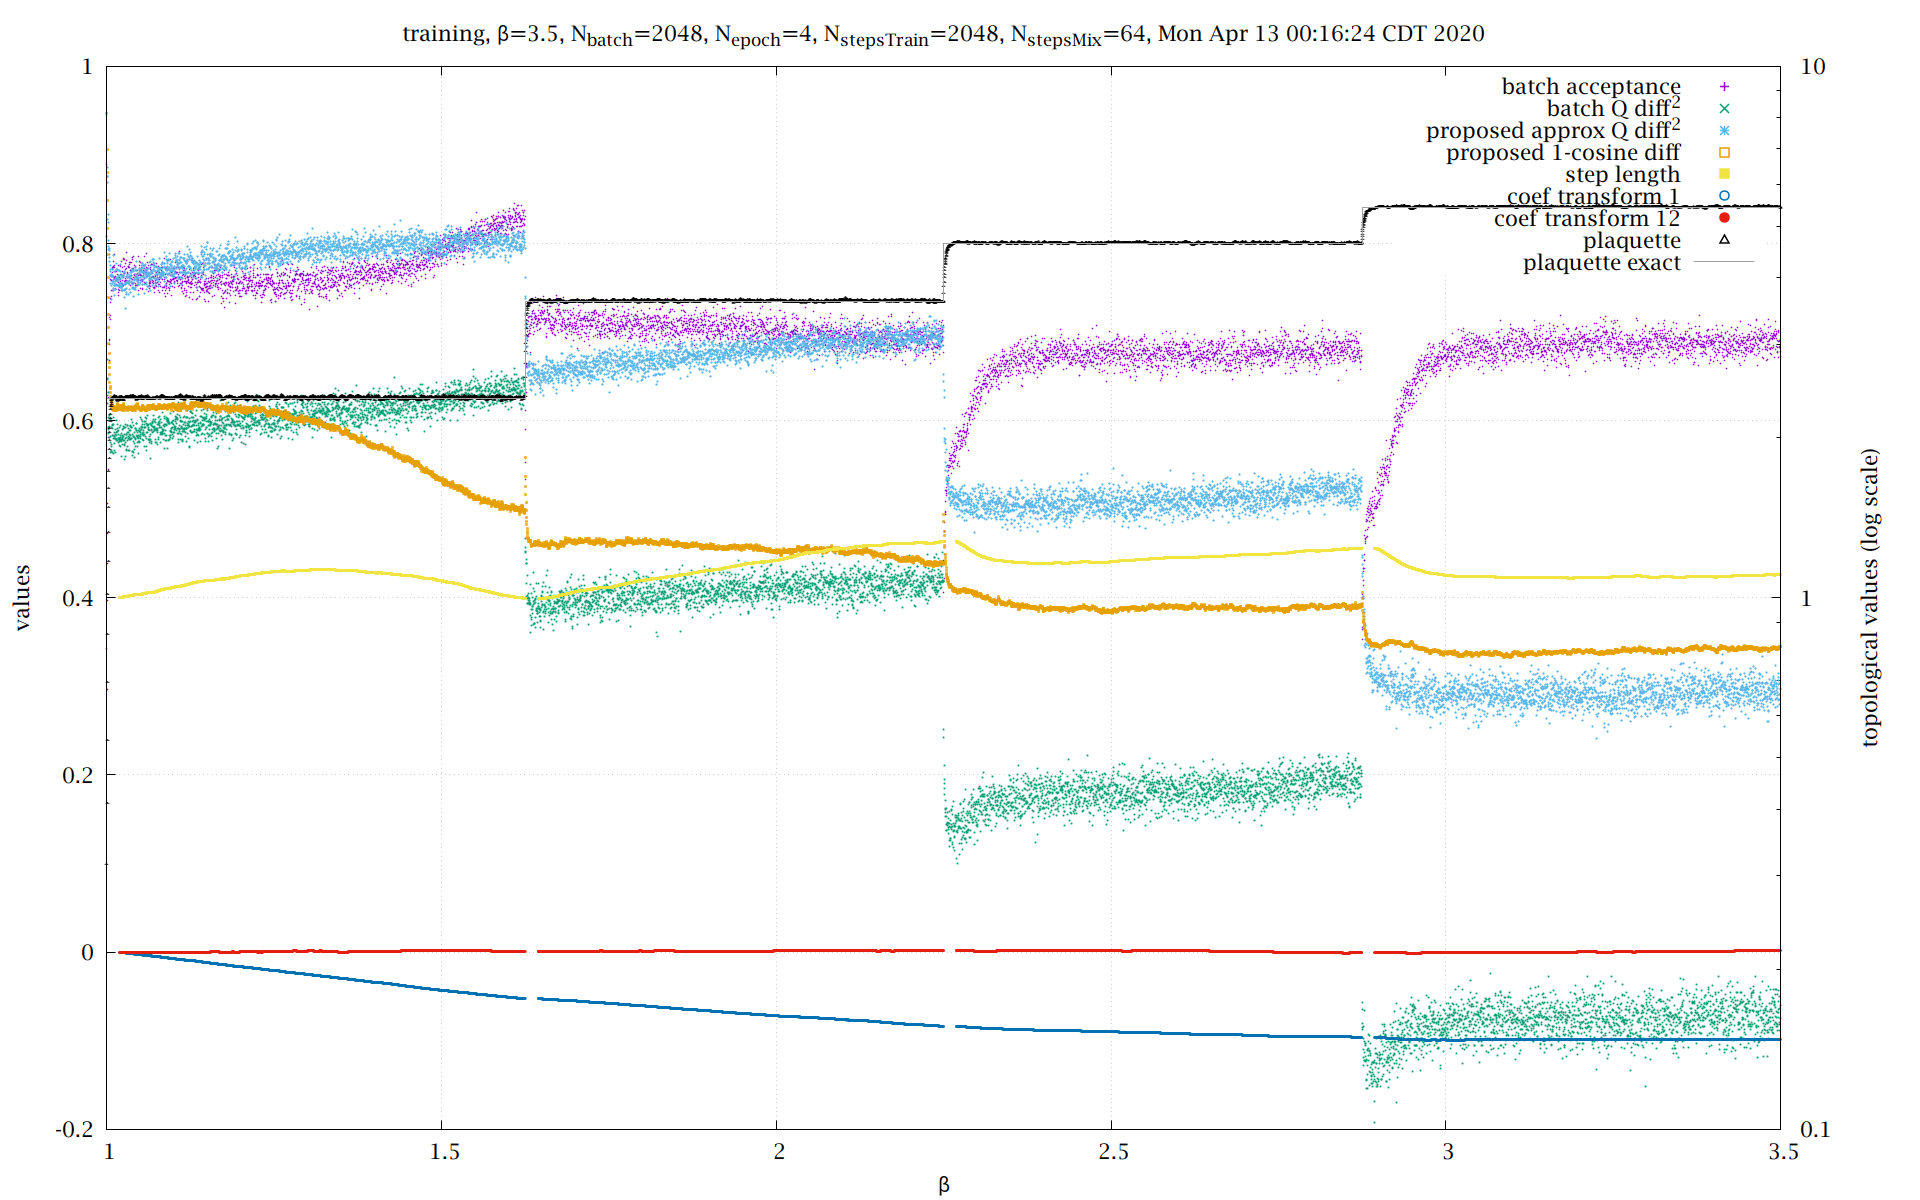
\includegraphics[width=\textwidth]{../t13.png}
	\caption{\label{training}Annealed training steps for $N=64$,
		at $β=1.625$, $2.25$, $2.875$, and $3.5$.}
\end{figure}

\begin{figure}
	\centering
	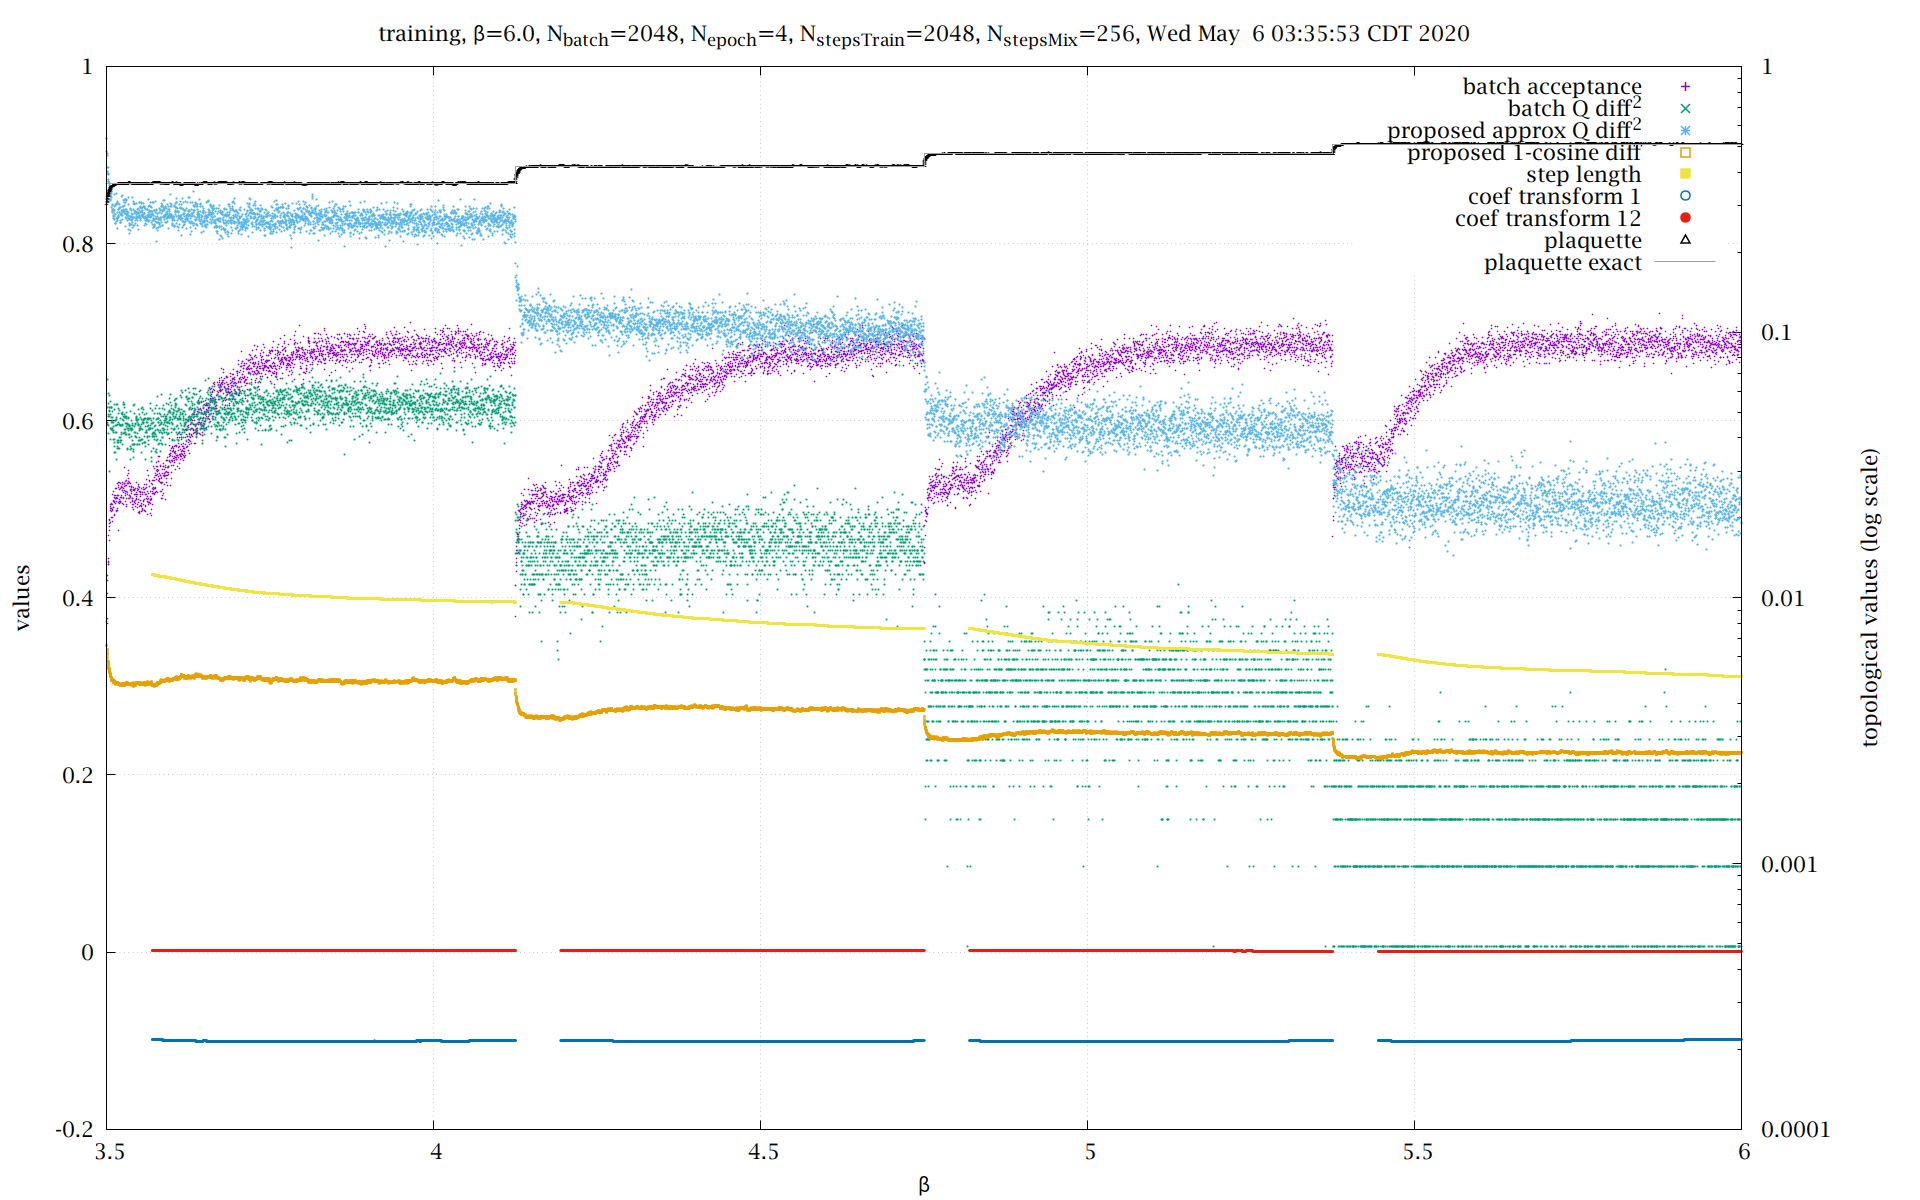
\includegraphics[width=\textwidth]{../t28.png}
	\caption{\label{training-b6}Continued annealed training steps for $N=64$,
		at $β=4.125$, $4.75$, $5.375$, $5.375$, and $6.0$.}
\end{figure}

Figure~\ref{topo-diff-n64} and \ref{topo-diff-n64-b6} show the root-mean-squared
difference of topological charges of consecutive Markov states over 1024 parallel
Markov chains started from random, with thermalizations removed.
The system is of size $N=64$, corresponding to the training system size,
and $β=1.625$, $2.25$, $2.875$, $3.5$, and $6.0$.

\begin{figure}
	\centering
	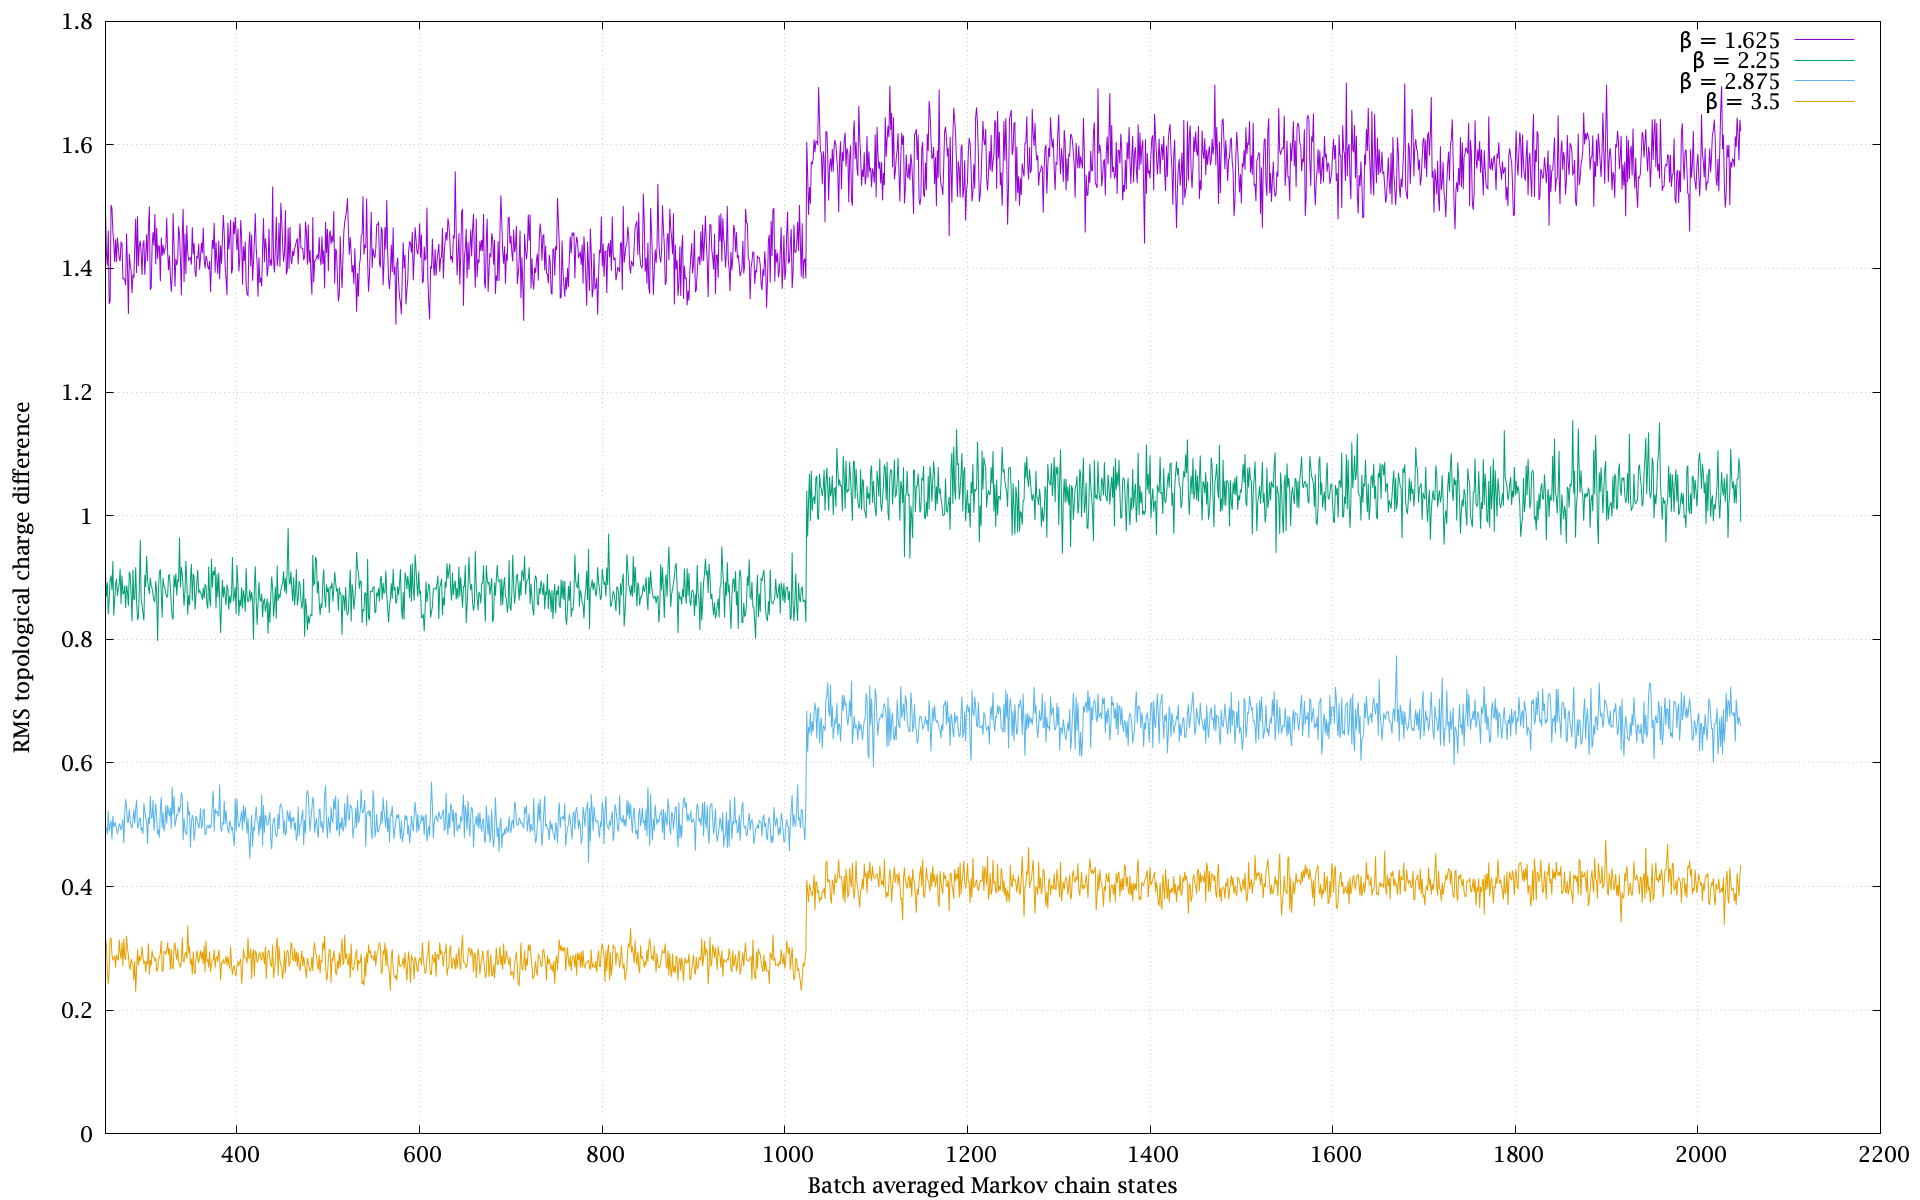
\includegraphics[width=\textwidth]{../topodiffN64.png}
	\caption{\label{topo-diff-n64}Topological charge change rate at $N=64$,
		at $β=1.625$, $2.25$, $2.875$, and $3.5$,
		with traditional HMC (trajectories before 1024)
		and field transformation HMC (after 1024).}
\end{figure}

\begin{figure}
	\centering
	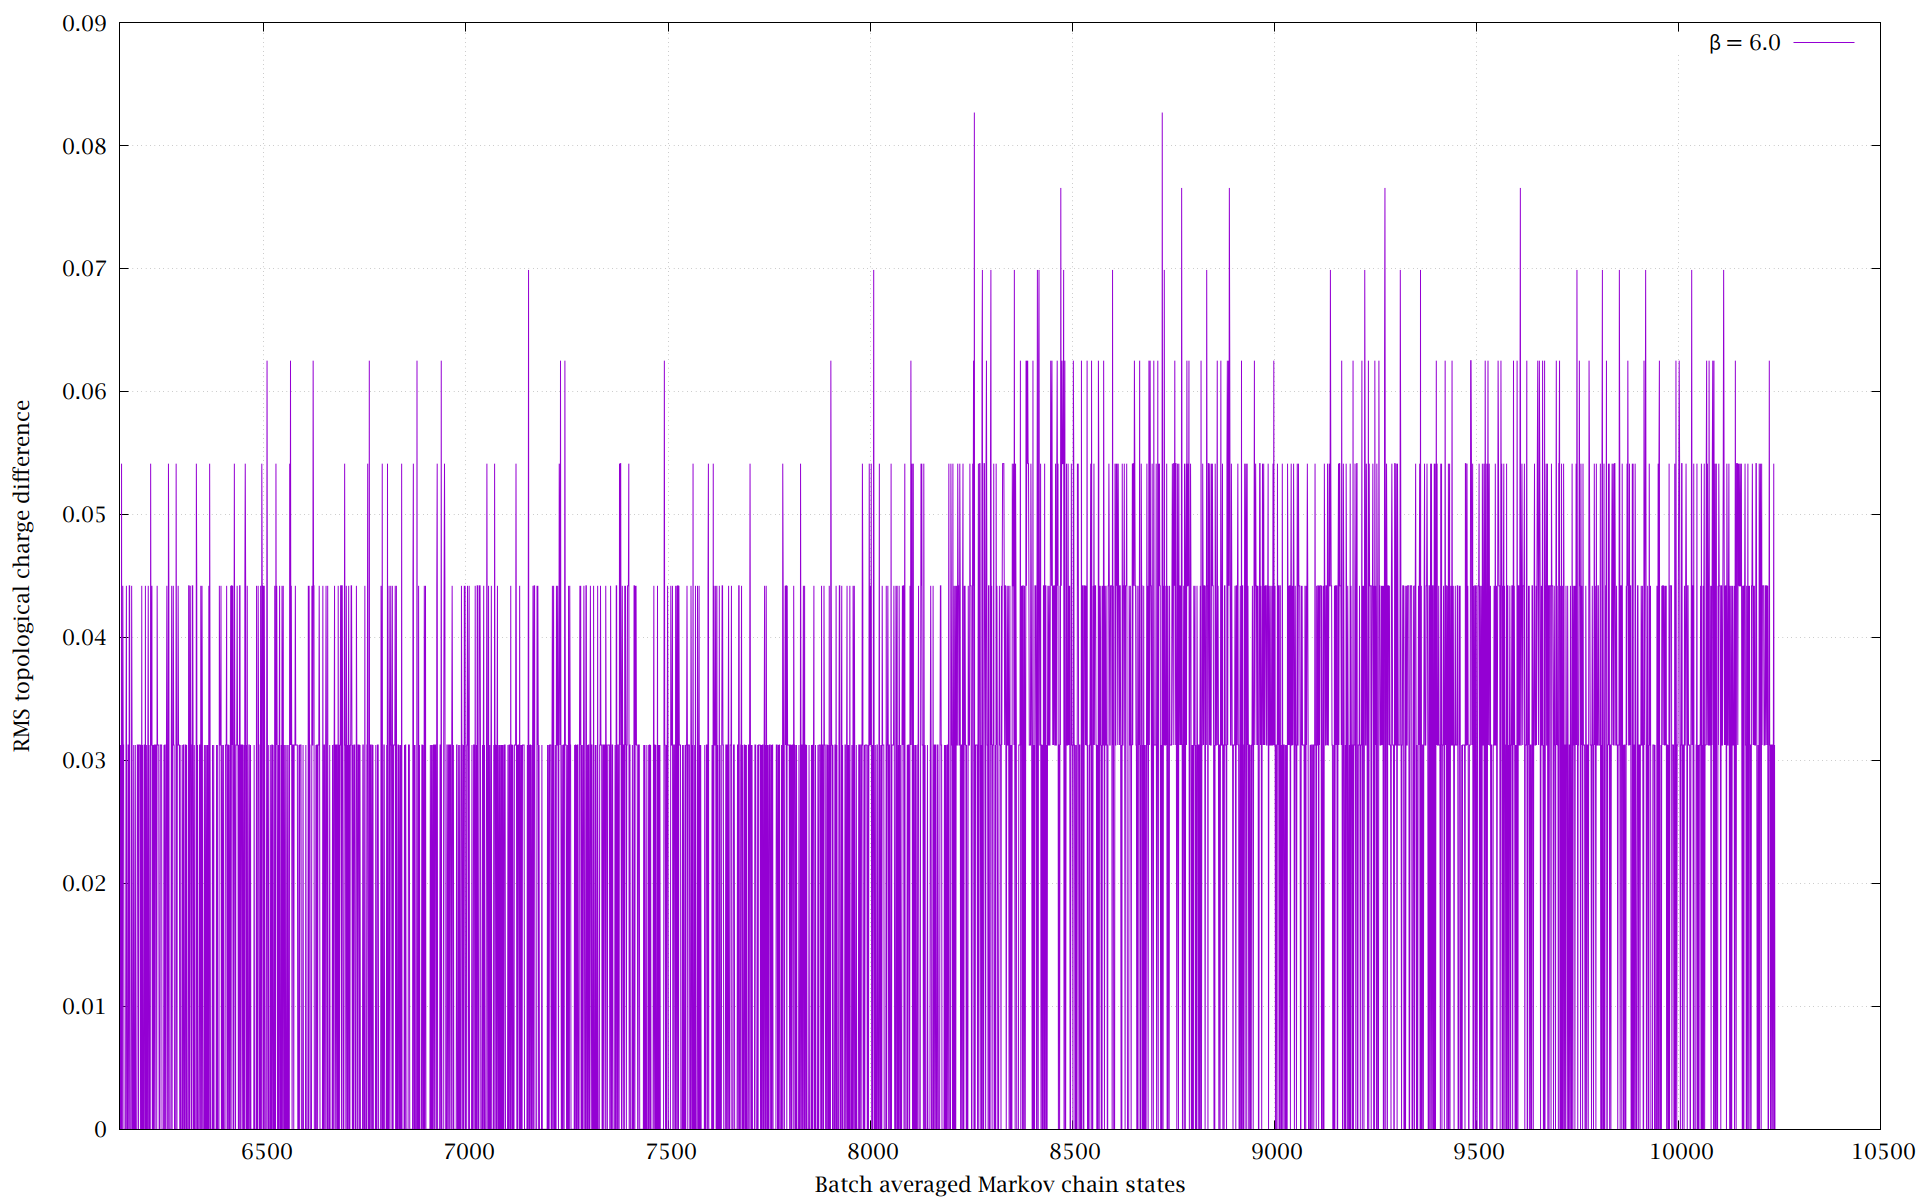
\includegraphics[width=\textwidth]{../topodiffN64_b6.png}
	\caption{\label{topo-diff-n64-b6}Topological charge change rate at $N=64$, $β=6.0$,
		with traditional HMC (trajectories before 8192)
		and field transformation HMC (after 8192).}
\end{figure}

We use the same parameters trained from $N=64$ to apply to a system of size $N=256$.
We reduce the leapfrog step size to be half of the trained value to get a good acceptance rate.
The resulting root-mean-squared difference of topological charges of consecutive Markov states
over 256 parallel Markov chains are in figure~\ref{topo-diff-n256} for $β=3.5$ and
figure~\ref{topo-diff-n256-b6} for $β=6.0$.
We change the number of leapfrog steps from $10$ (used in training) to $20$ and $30$.
Figure~\ref{topo-evo-n256} shows the evolutions of topological charges in
a few individual Markov chains at $β=3.5$ using 10 leapfrog steps per trajectory.
Figure~\ref{topo-evo-n256-b6} shows the same for $β=6.0$ using 10 leapfrog steps per trajectory,
while figure~\ref{topo-evo-n256-b6-s30} is for $β=6.0$ using 30 leapfrog steps per trajectory.

\begin{figure}
	\centering
	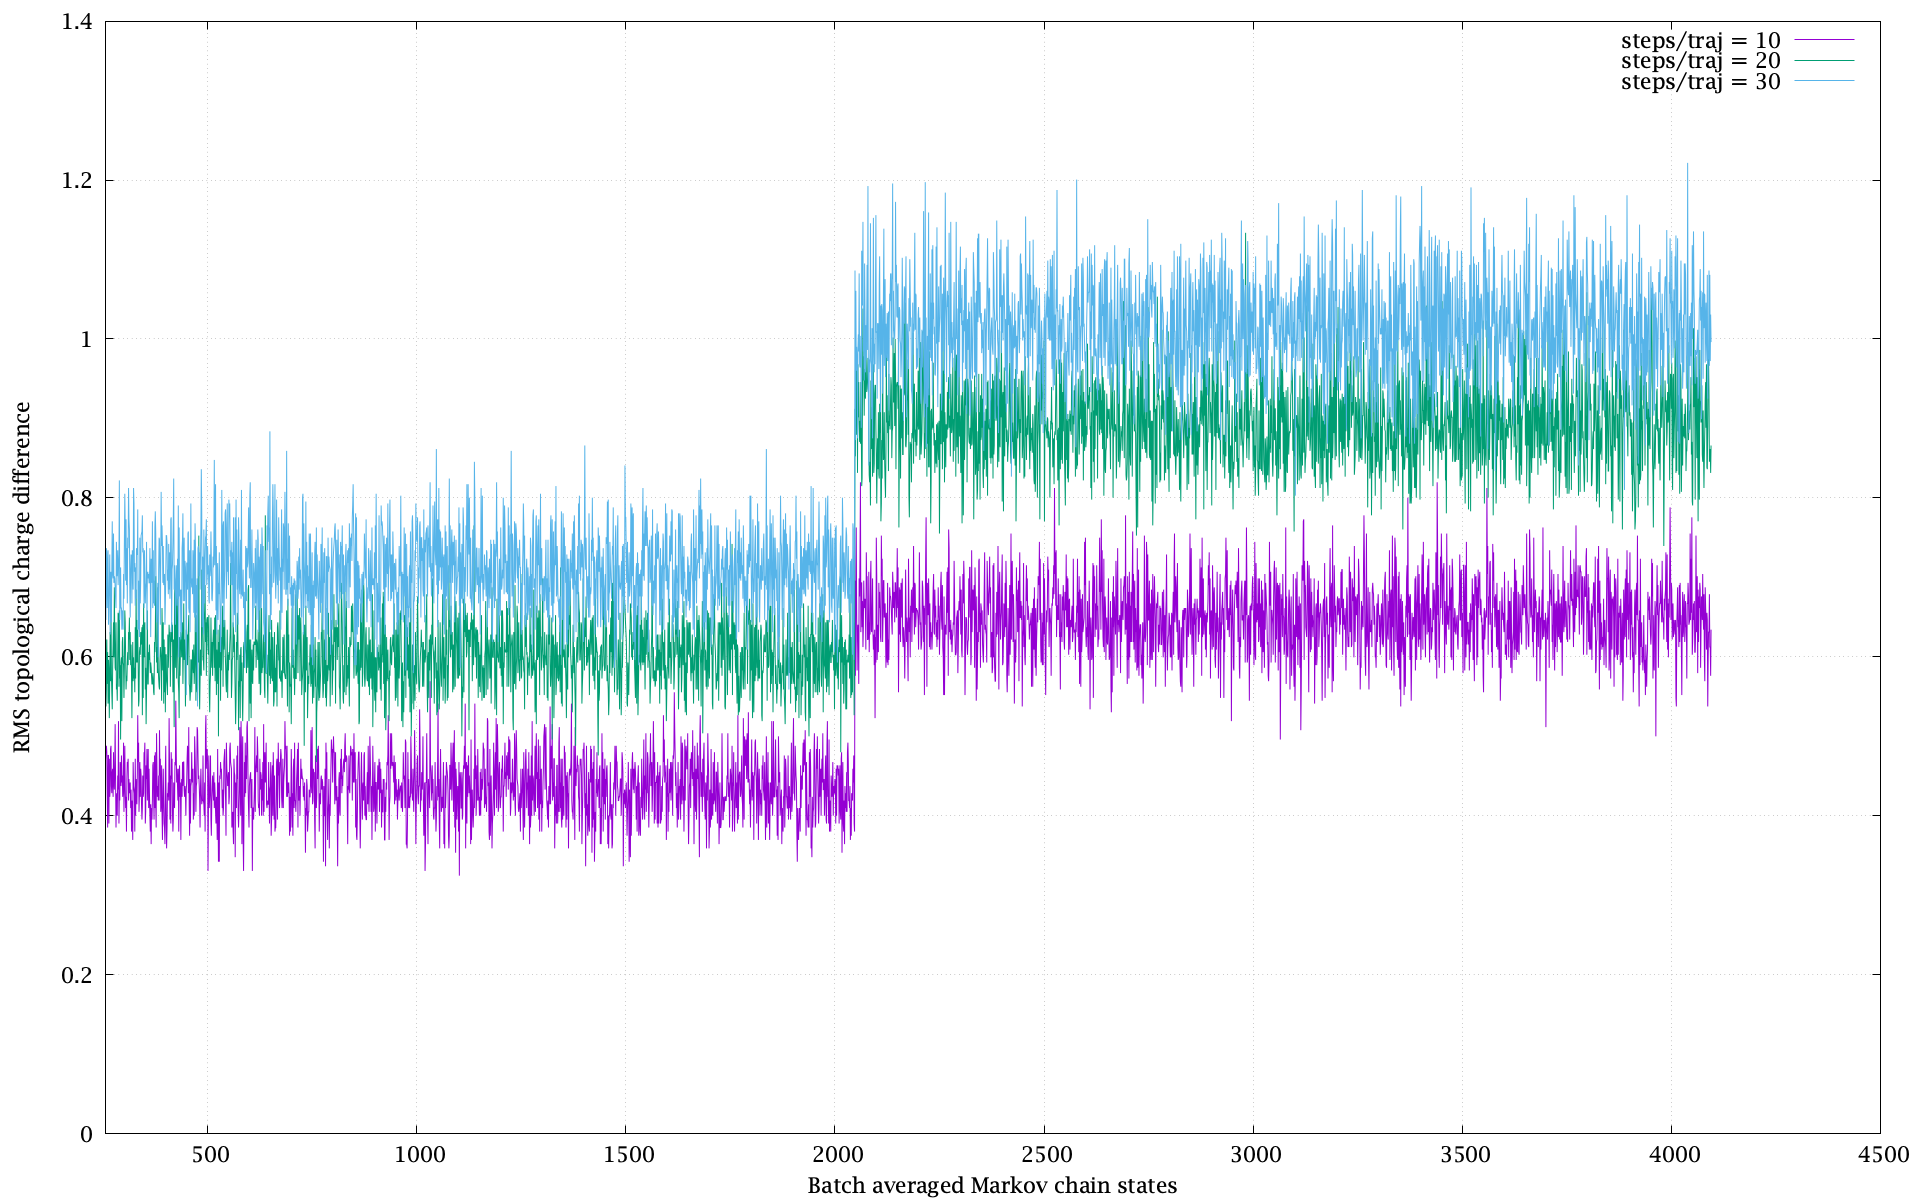
\includegraphics[width=\textwidth]{../topodiffN256.png}
	\caption{\label{topo-diff-n256}Apply trained parameters from $N=64$ to $N=256$, $β=3.5$,
		with traditional HMC (trajectories before 2048)
		and field transformation HMC (after 2048).}
\end{figure}

\begin{figure}
	\centering
	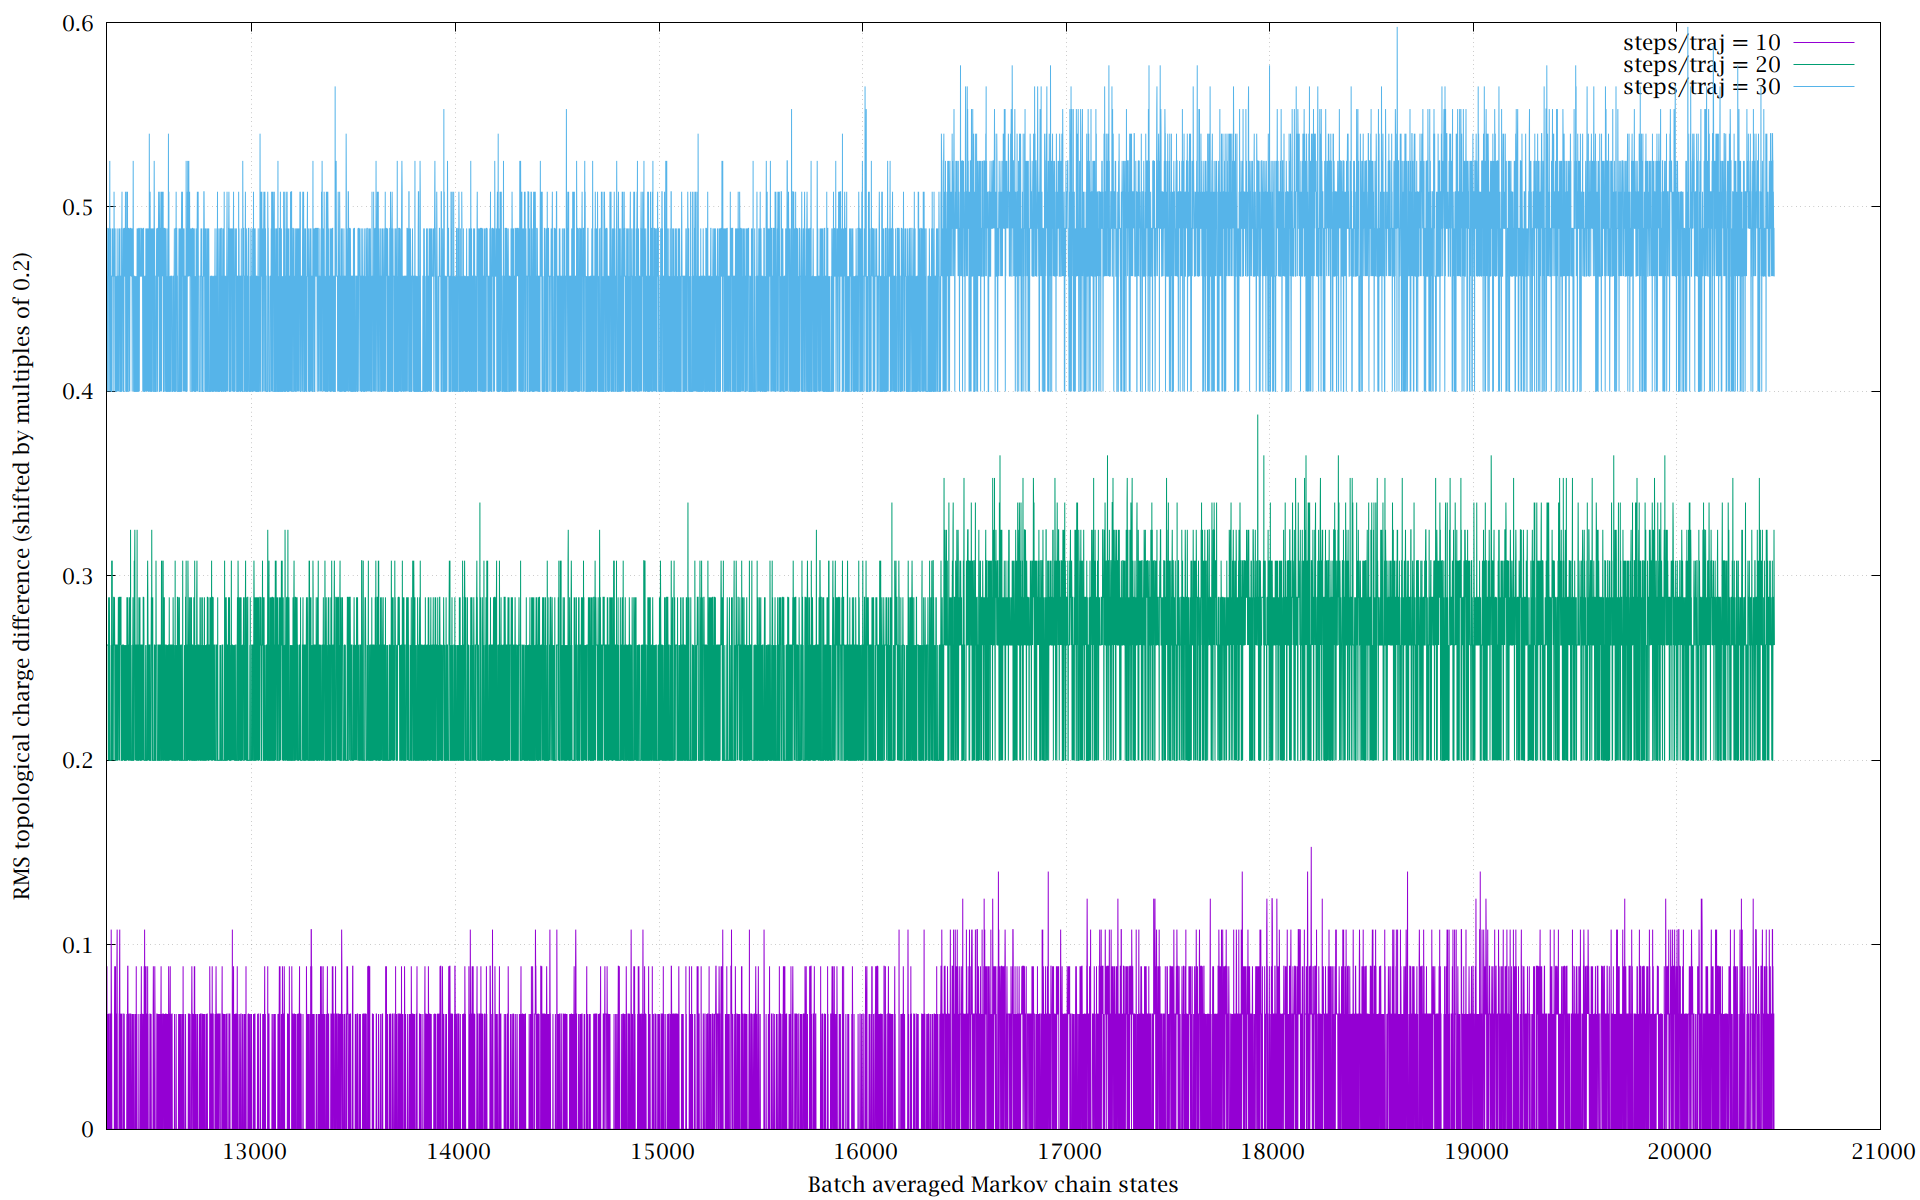
\includegraphics[width=\textwidth]{../topodiffN256_b6.png}
	\caption{\label{topo-diff-n256-b6}Apply trained parameters from $N=64$ to $N=256$, $β=6.0$,
		with traditional HMC (trajectories before 16384)
		and field transformation HMC (after 16384).}
\end{figure}

\begin{figure}
	\centering
	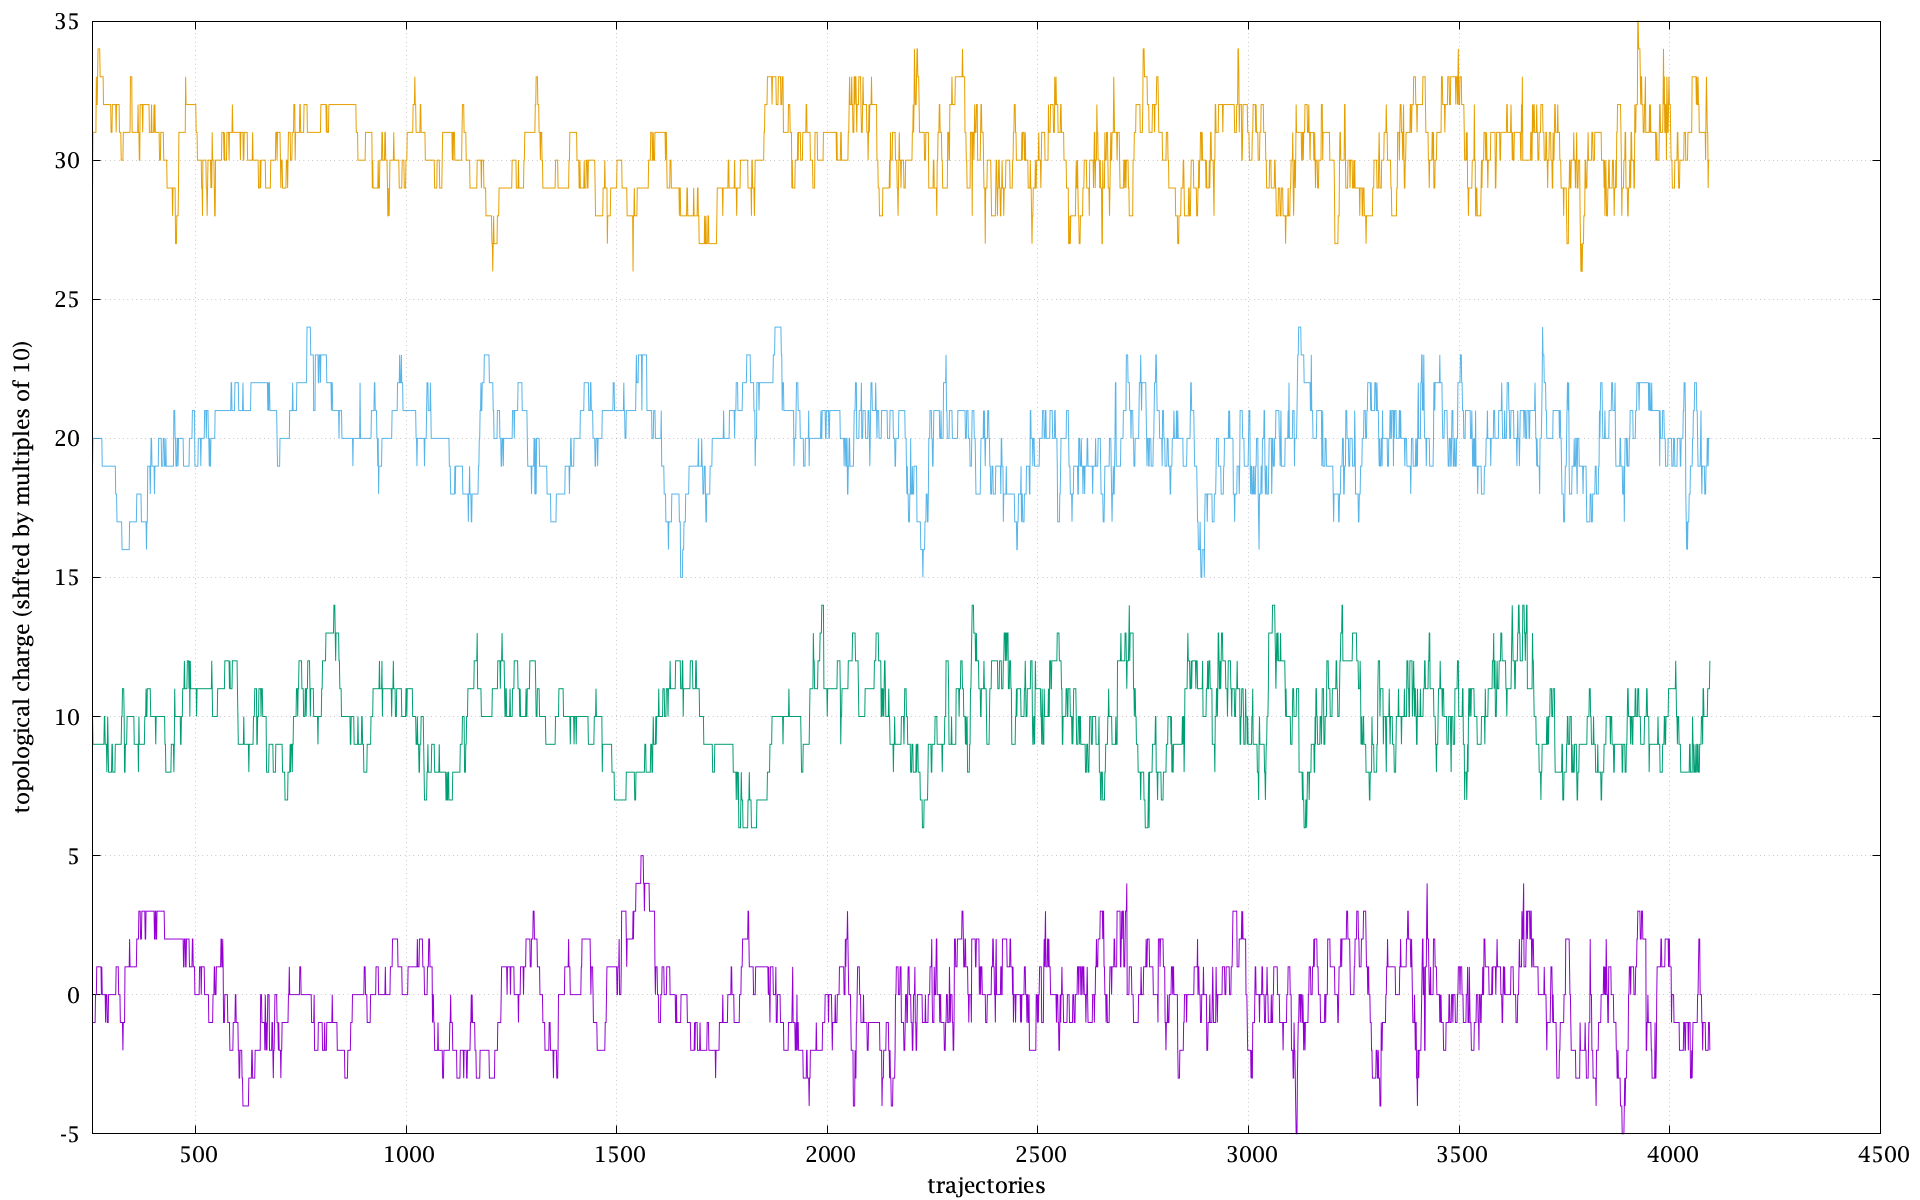
\includegraphics[width=\textwidth]{../topoevoN256.png}
	\caption{\label{topo-evo-n256}Individual MC evolution after
		applying trained parameters from $N=64$ to $N=256$, $β=3.5$,
		with traditional HMC (trajectories before 2048)
		and field transformation HMC (after 2048).}
\end{figure}

\begin{figure}
	\centering
	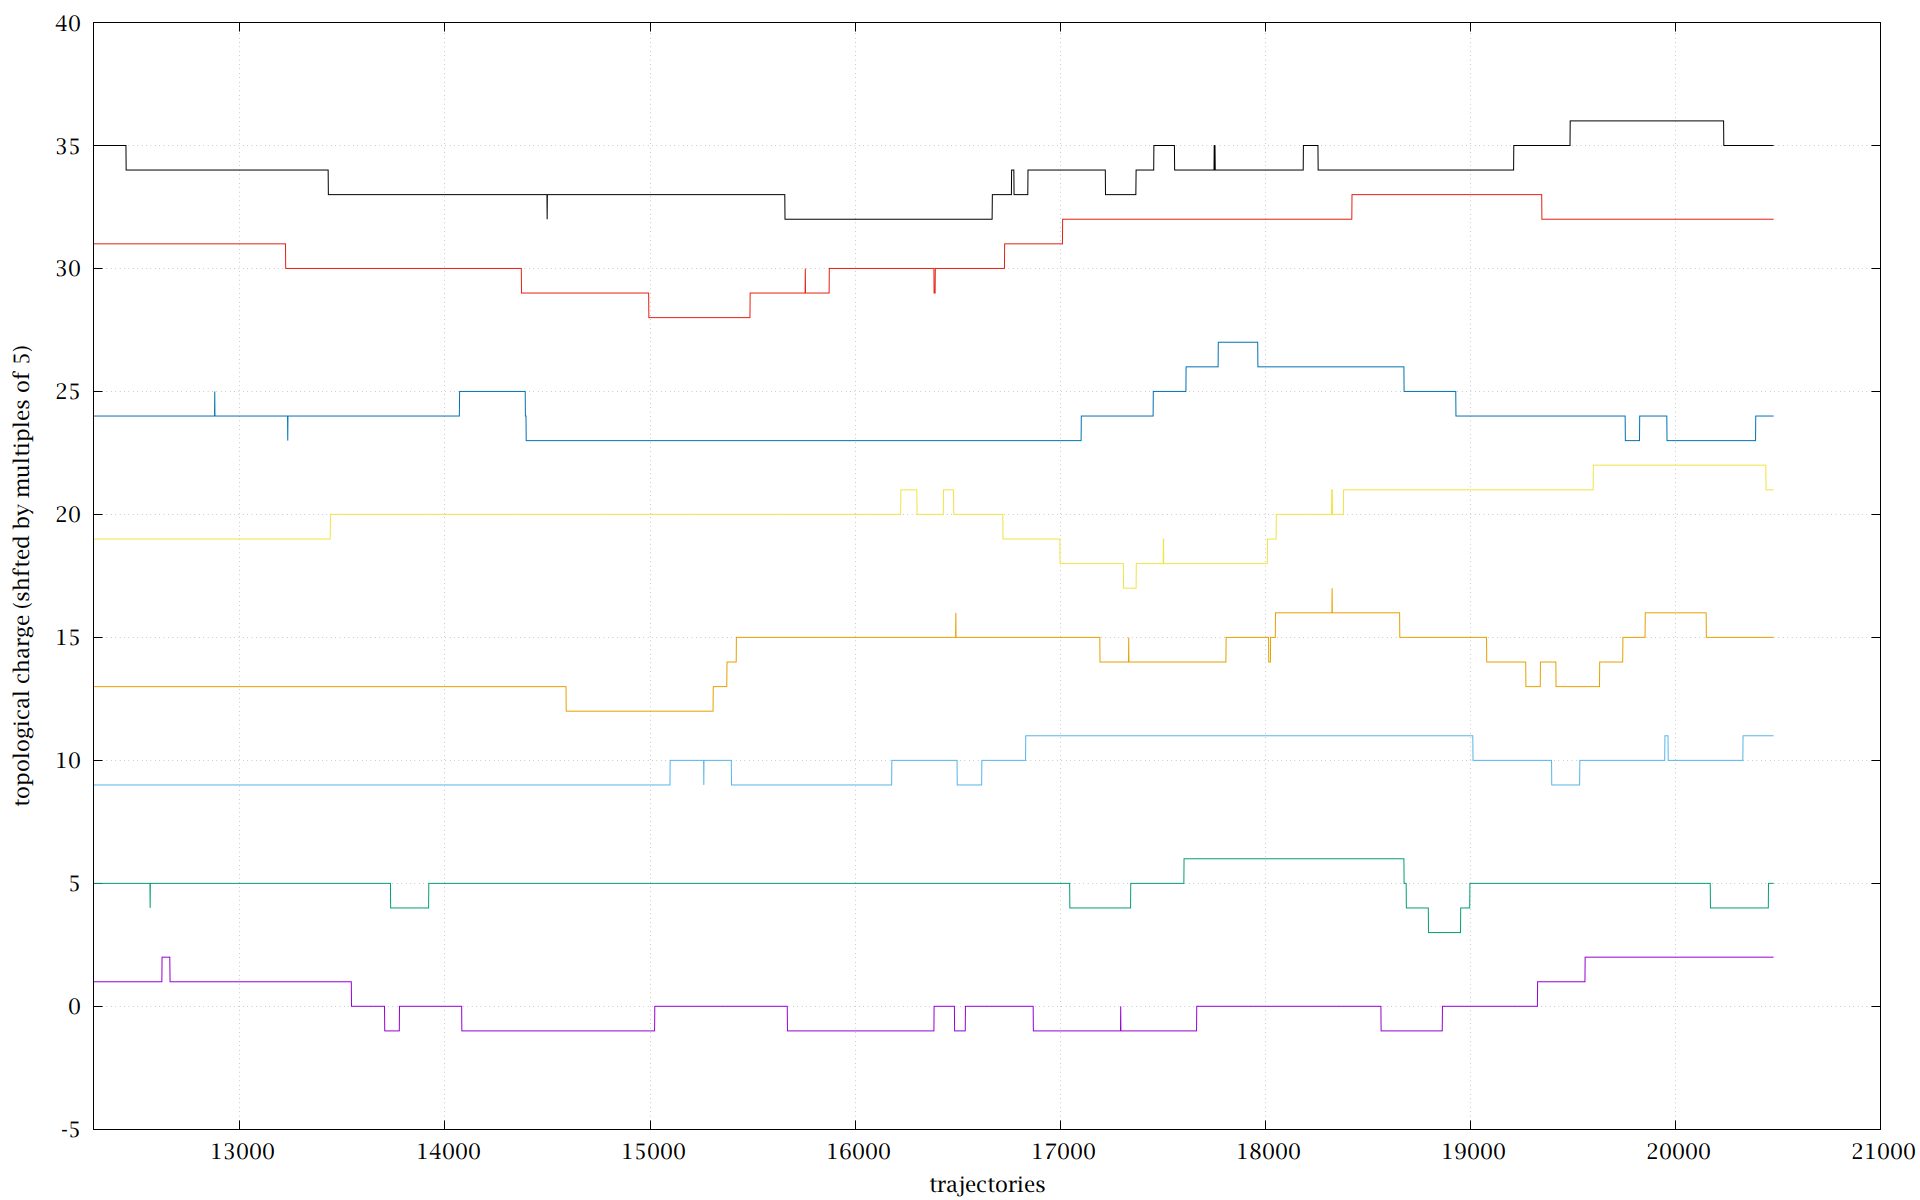
\includegraphics[width=\textwidth]{../topoevoN256_b6.png}
	\caption{\label{topo-evo-n256-b6}Individual MC evolution after
		applying trained parameters from $N=64$ to $N=256$, $β=6.0$,
		with traditional HMC (trajectories before 16384)
		and field transformation HMC (after 16384).}
\end{figure}

\begin{figure}
	\centering
	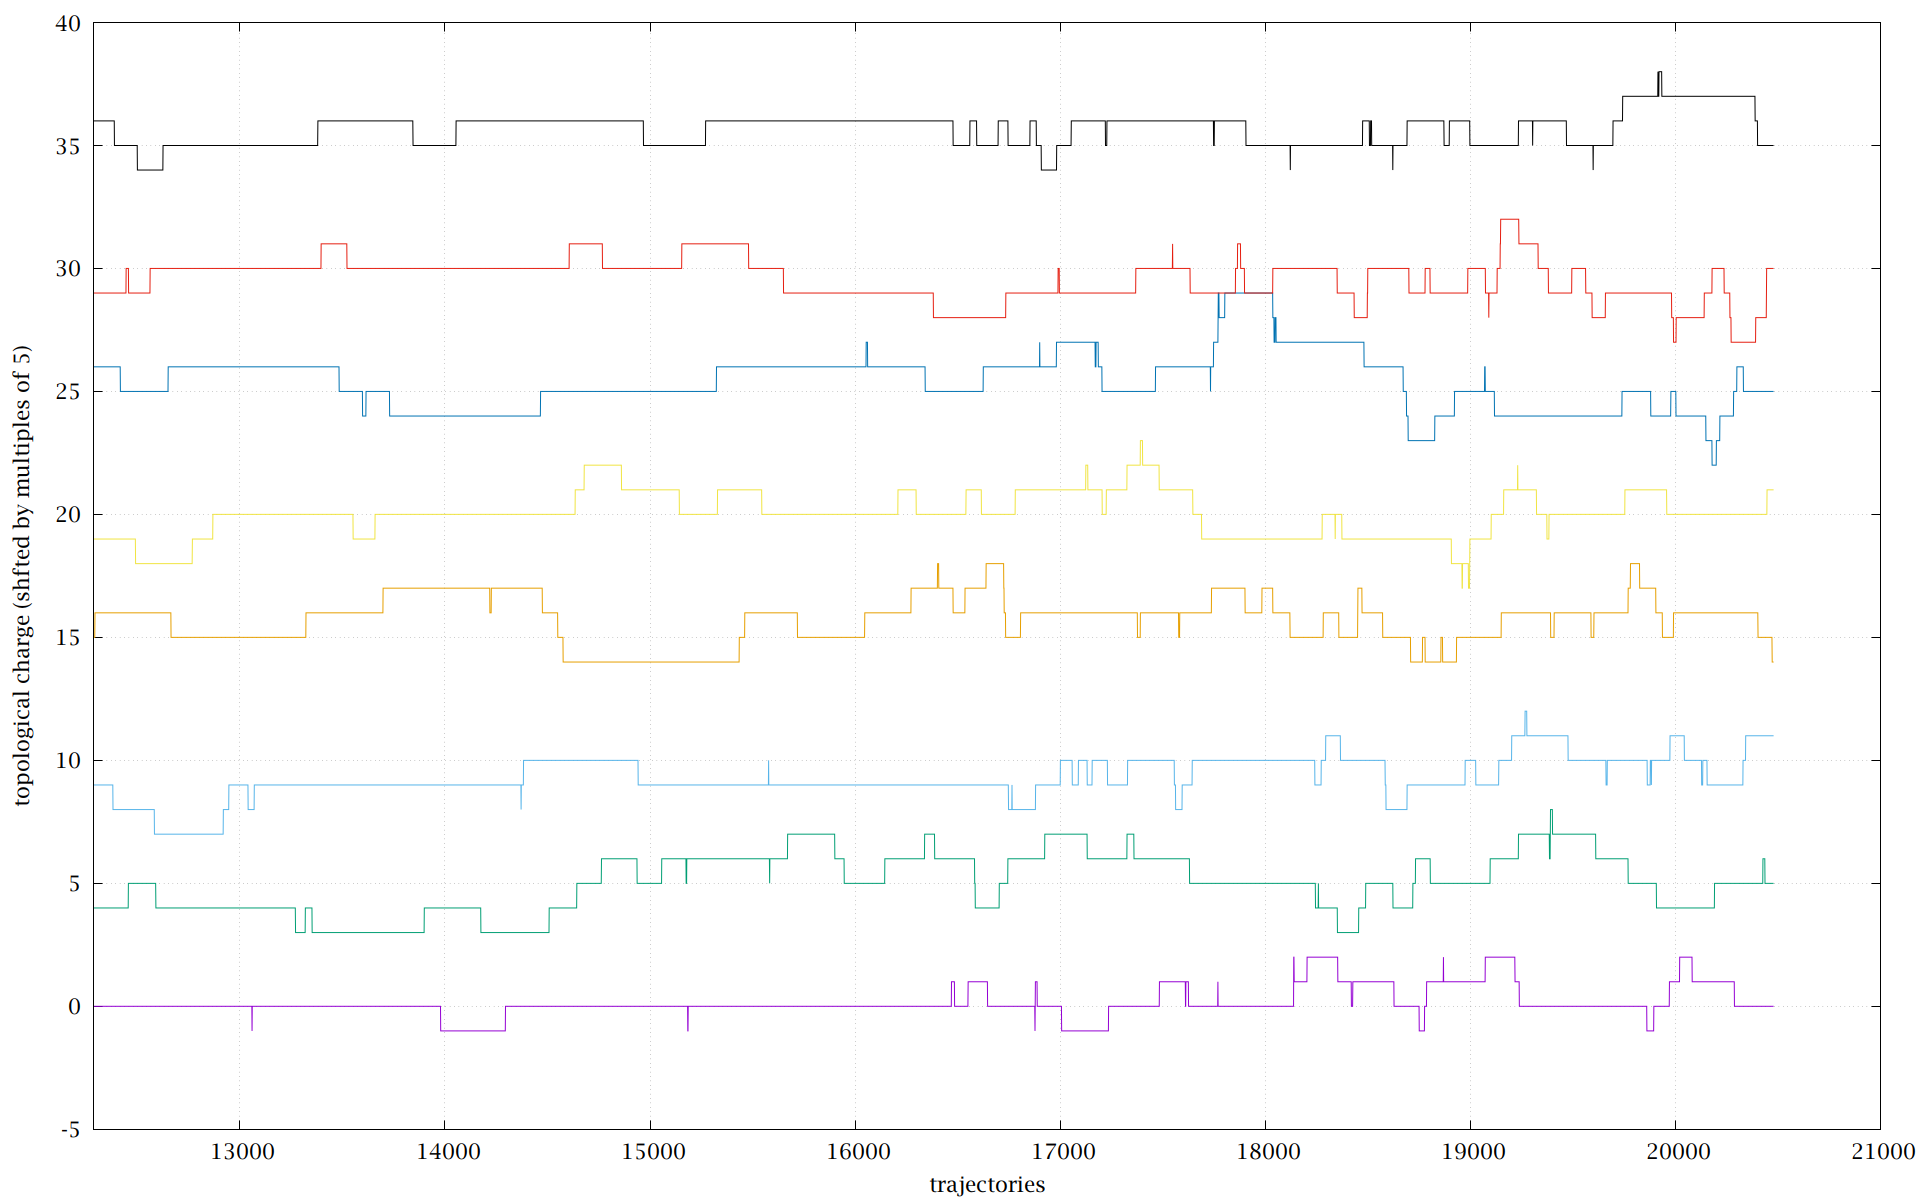
\includegraphics[width=\textwidth]{../topoevoN256_b6_n30.png}
	\caption{\label{topo-evo-n256-b6-s30}Individual MC evolution after
		applying trained parameters from $N=64$ to $N=256$, $β=6.0$,
		using 30 steps per trajectory,
		with traditional HMC (trajectories before 16384)
		and field transformation HMC (after 16384).}
\end{figure}

